\chapter{Model Analysis}
\label{sec:kldaAnalysis}

Any proposed model such as the one detailed in Chapter~\ref{sec:klda} can be analyzed either \textit{intrinsically} or \textit{extrinsically}, with or without reference to a particular task.   We evaluated standard LDA and cache-based language models extrinsically in Chapter 4 in the context of the keyword retrieval task, and we will evaluate our proposed cache-augmented topic model on the same extrinsic task in Chapter 7.  In this chapter, we begin by looking directly at intrinsic, observable properties of the model, but also examine model properties through extrinsic tasks such as language modeling and topic discovery.

%We devote this chapter to an intrinsic analysis of our proposed model.  
We estimate model parameters on informal speech corpora in a number of languages and consider the model behavior from different perspectives.  We first look at the convergence and consistence of the approximate inference process itself.  Given the stochastic nature of Gibbs sampling, we look at consistency and convergence across multiple iterations on the same corpora.  Next we look specifically of the repetition properties inferred by our model.  We ask whether the inferred cache properties correspond to our intuitions and related repetition phenomena of the data.   We then look at constructing a unigram language model from the learned topic distributions and look at perplexity behavior on held out data, contrasting this with standard LDA models on the same data.  Lastly, we use external topic discovery tasks to asses the quality of the `subject matter' topic distributions.

% as with the work on repetition, we want kappa to reflect repetition quantity of the corpus, but also want that to be useful for the interpolation task

\section{Convergence and Consistency}

In recent years, many approximate inference techniques have been well studied in the context of the standard LDA topic model, to include different implementations and optimizations (cf. \cite{hoffman2010online}, \cite{zhai2012mr}, \cite{yao2009efficient}).  One standard point of comparison is the \textit{convergence} of different algorithms or models in terms of some metric.  Convergence speaks to both the stability of the model and the efficiency of inference algorithm.  Typically convergence can be expressed as the \textit{likelihood} (or derived metrics, \textit{log-likelihood} or \textit{perplexity}) of either the training data or a held out data set under the model.

Additionally, because of the stochastic nature of Gibbs Sampling (and other MCMC) approaches we can ask how \textit{consistent} different runs of the inference algorithm are for LDA or for our cache-augmented model.  To illustrate  both consistency and convergence of our proposed model, we perform 5 trials of parameter estimation on a number of similarly sized speech corpora.  We can show that in terms of consistency, both LDA and our cache-augmented model are equivalently stable across trials and exhibit similar convergence behavior over time.  We also analyze the convergence and consistency specifically of the $\kappa^{(d)}$ parameter under different corpora and number of topics.  Again, we can show the parameter estimation converges and is stable across trials, but as intuition suggests, the behavior differs across languages.

In this chapter and in the next we focus primarily on low-resource speech recognition and retrieval scenarios.  As before we utilize Limited Language Pack (Limited LP) resources from the IARPA {\small Babel} program, which contain only 10 hours of transcribed audio.  The languages we consider in this chapter include Turkish, Tagalog, Vietnamese, Zulu and Tamil.\footnote{Language collection releases babel105b-v0.4, babel106-v0.2g, babel107b-v0.7, babel206b-v0.1e, and babel204b-v1.1b respectively.}  
% NOTE and for task evaluation which require labels, we use spanish and enlgish
For interpretability of topics and cached words, we also estimate models on the CallHome Spanish corpus from LDC, which contains roughly 14 hours of transcribed conversational speech \cite{callhome}, LDC's Fisher Spanish transcripts \cite{ldc2010}, with 178 hours of transcribed speech, and the 359 hour subset of LDC's Fisher English transcripts we previously used for Topic ID experiments.

\begin{table}[t]
\begin{center}
   \begin{tabular}{lrrrr}\toprule
   \textbf{Corpus}  &  \textbf{Docs} & \textbf{Utts/Doc} & \textbf{Tokens/Doc} & \textbf{Tokens/Utt}\\ \midrule
   Turkish & 128 & 81.45 & 565.17 & 6.94 \\
   \rowcolor{blue!5} Tagalog & 132 & 87.52 & 534.02 & 6.10 \\
   Vietnamese & 126 & 80.71 & 932.86 & 11.56 \\
   \rowcolor{blue!5}   Zulu & 124 & 85.20 & 520.45 & 6.12 \\
   Tamil & 125 & 85.77 & 601.57 & 7.01 \\
   \rowcolor{blue!5}   Spanish (CallHome) & 160 & 107.51 & 903.84 & 8.41	\\
   Spanish (Fisher) & 1286 & 159.25 & 986.32 & 6.19 \\
   \rowcolor{blue!5} English (Fisher) & 2060 & 189.31 & 1899.05 & 10.03 \\\bottomrule
  \end{tabular}
\caption[Corpus sizes, conversational speech]{Corpus sizes in terms of documents, utterances, and word tokens\label{fig6:cstats}}
\end{center}

\end{table}

Corpus statistics are provided in Table~\ref{fig6:cstats}.  The Babel corpora are roughly all of the same size in terms of number and length (number of utterances) of documents.  For speech corpora, we generally use silence-segmented utterances, roughly corresponding to a single conversation turn, instead of sentences.  Sentences are generally not well delineated in speech transcripts.  The Spanish corpora contain noticeably longer documents at least in terms of the number of utterances.  English contains more words per utterance.  There is some variance in terms of the number of word tokens per utterance, particularly for Vietnamese, which as has been mentioned was transcribed with syllable level word tokens.  %This, as opposed to document length we might expect to be more a language-specific property.
%Likelihood  LDA (1, 2 gram) vs kLDA

\begin{figure}
\begin{center}
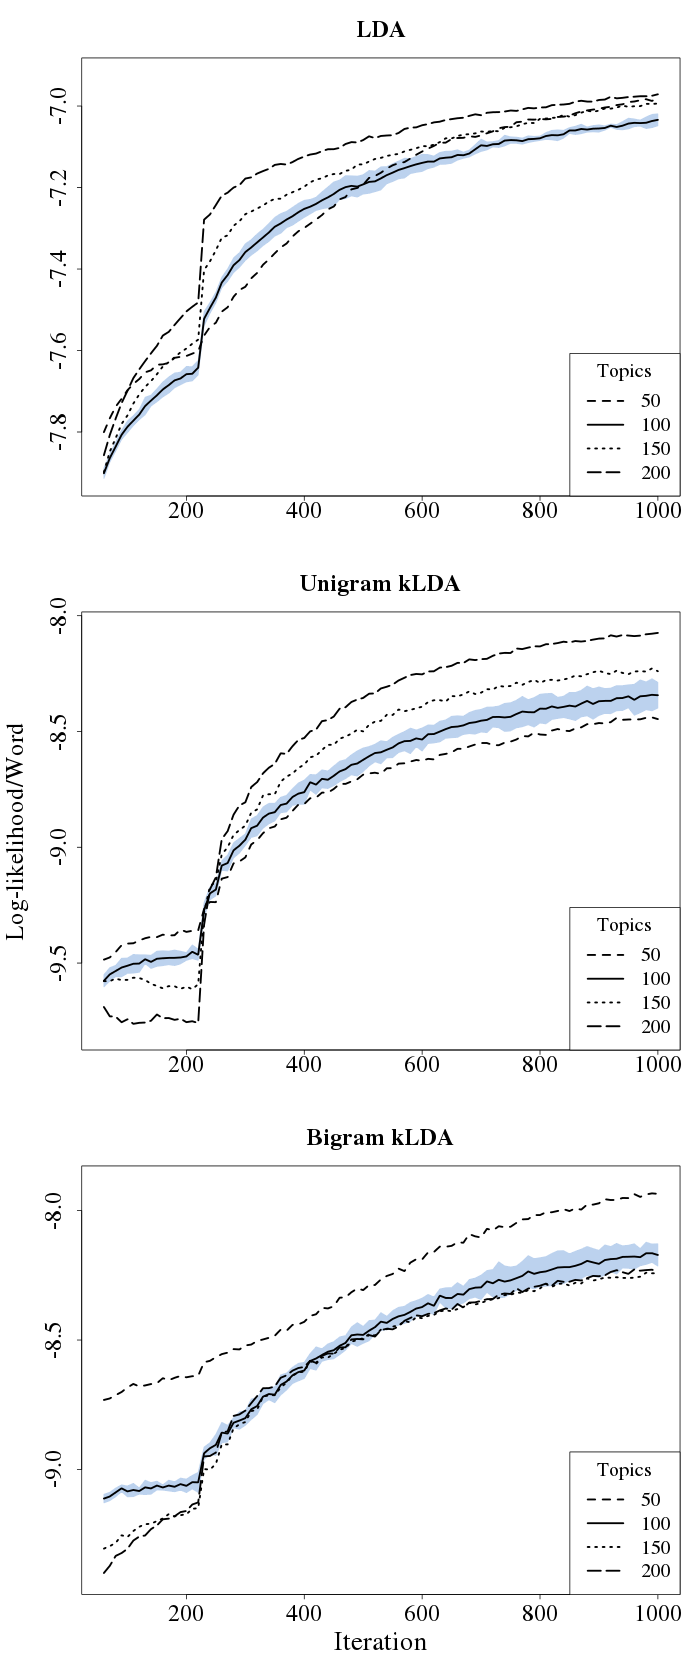
\includegraphics[width=0.5\textwidth]{graphs/ch6/ll/chsp-lda-ll.png}
\end{center}
\caption[Log-likelihood convergence, CallHome Spanish]{Model log-likelihood convergence over sampling process for CallHome Spanish transcripts.\label{fig6:llCallHome}}
\end{figure}

For each corpus we analyze the training log-likelihood (per word token) over 1000 iterations of Gibbs Sampling, and averaged over 5 independent trials.  We contrast the Mallet implementation of LDA with our proposed cache-augmented model (abbreviated $\kappa$LDA) with either unigram or bigram cache.  We also consider topic mixtures (under all models) of \{50,100,150,200\}.  

Figure~\ref{fig6:llCallHome} illustrates the convergence of the per-word log-likelihood over 1000 iterations for each model condition when training on the CallHome Spanish corpus.  The shaded area around the 100 topic condition indicates $\pm$ 1 sample standard deviation of the log-likelihood measurement across the 5 trials.   The tightness of the log-likelihood estimates over all iterations indicates that sampling under our cache-augmented model is roughly as stable as LDA across trials.  

% generated by graphs/ch6/ll2.R

\begin{figure}
\begin{center}
\subfloat[Vietnamese\label{fig6:llVietnamese}]{%
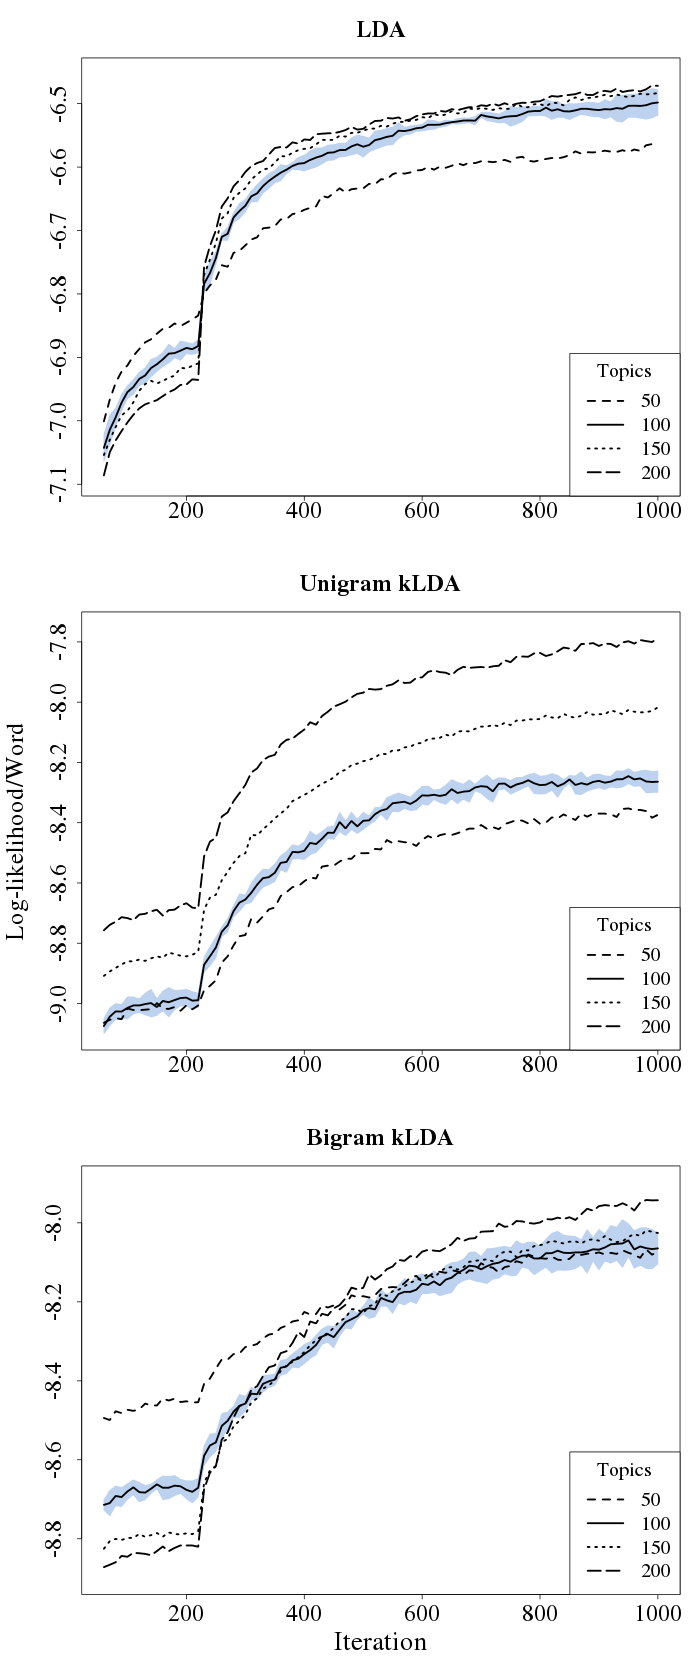
\includegraphics[width=0.45\textwidth]{graphs/ch6/ll/vietnamese-lda-ll.png}
}
\hfill
\subfloat[Turkish\label{fig6:llTurkish}]{%
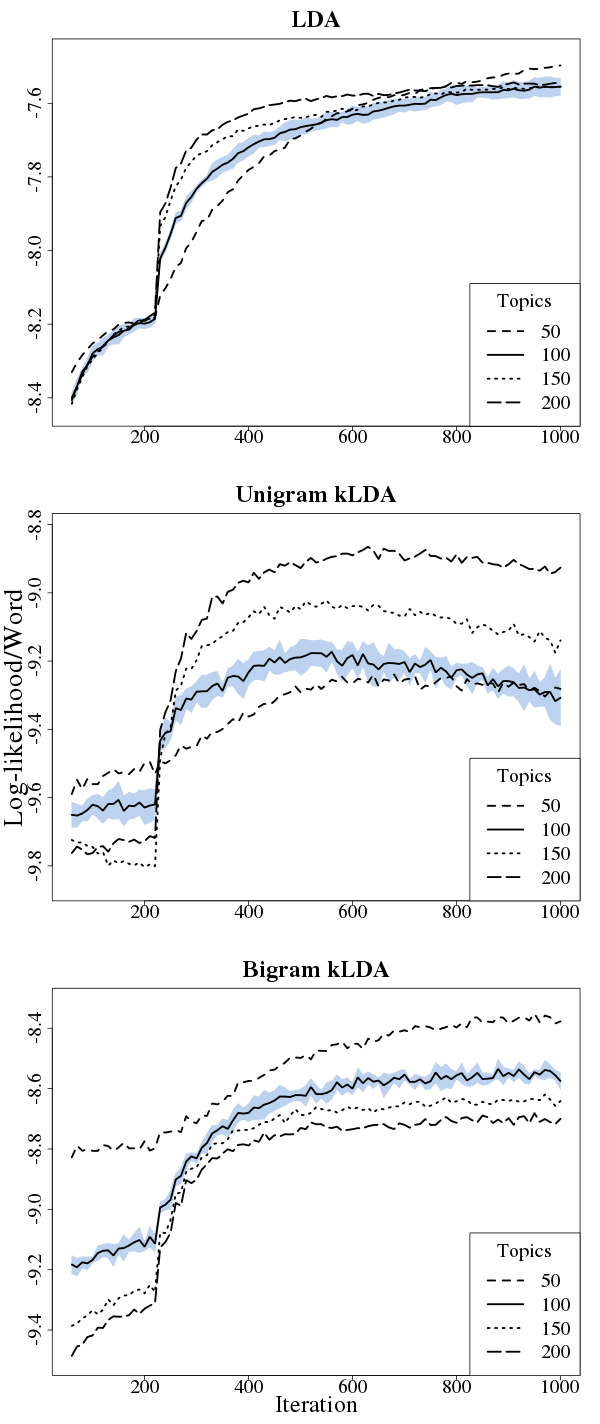
\includegraphics[width=0.45\textwidth]{graphs/ch6/ll/turkish-lda-ll.png}
}
\end{center}
\caption[Log-likelihood convergence, Babel Corpora]{Model log-likelihood convergence over sampling process for Babel Vietnamese and Turkish transcripts.\label{fig6:llComp}}
\end{figure}


For the sake of comparison we present the convergence figures for the Babel Vietnamese and Turkish (cf. Figures~\ref{fig6:llVietnamese},~\ref{fig6:llTurkish}).  Indeed from a convergence perspective, the two behave similarly under standard LDA.  However the sampling becomes significantly less smooth moving from Vietnamese to Turkish.  For completeness, we include convergence figures for all corpora in Appendix~\ref{sec:llconverge}.  With respect to log-likelihood convergence, in all cases the trajectory consistently changes around iteration 250, which is consistent with the application of the hyperparameter re-estimation from Wallach et al.\cite{wallach2009} from that point on in all trials.

Alternatively, if we look at the absolute model log-likelihood we see that the cache-augmented models underperform standard LDA in both the unigram and bigram cache cases.  However we will re-visit this shortly in terms of language model perplexity.  Table~\ref{fig6:llstats} details the likelihood values as well as the sample standard deviation across trials (in parentheses) under all model conditions.  Irrespective of the absolute value, the low variance across trials is a quantitative indication of the likelihood stability of both LDA and our proposed variants.  Included are the results for the 100 topic case, with results for the 50, 150, and 200 topic case provided in full in Appendix~\ref{sec:llconverge}.

\begin{table}[t]
\begin{center}
   \begin{tabular}{lrrr}\toprule
   \textbf{Corpus} & \textbf{LDA} & \textbf{$\kappa$LDA-1} & \textbf{$\kappa$LDA-2}\\ \midrule
Turkish &  -7.554 (0.02) & -9.173 (0.04) & -8.535 (0.02) \\
Tagalog &  -6.523 (0.02) & -8.210 (0.03) & -7.910 (0.04) \\
Vietnamese & -6.498 (0.01) & -8.245 (0.03) & -8.044 (0.03) \\
Zulu &  -7.887 (0.02) & -9.912 (0.03) & -8.594 (0.03) \\
Tamil &  -7.887 (0.02) & -9.993 (0.04) & -8.853 (0.03) \\
Spanish (CallHome) &  -7.034 (0.02) & -8.341 (0.04) & -8.164 (0.04) \\
Spanish (Fisher) & -7.505 (0.01) & -8.381 (0.01) & -8.270 (0.03) \\
 \bottomrule
  \end{tabular}
\caption[Model log-likelihood per word]{Model log-likelihood per word after 1000 iterations, averaged over 5 runs, sample standard deviation in parenthesis.\label{fig6:llstats}}
\end{center}
\end{table}


\section{Repetition}
\label{sec:kldaRepetition}

The next manner in which we can look intrinsically at the parameters output by our cache-augmented model is by analyzing to what extent the latent variables capture token \textit{repetition} within various corpora.  Within our model, repetition is captured by the cache indicator variables $k_{d,i}$ and per-document cache prior $\kappa^{(d)}$.  We expect the former to be assigned to word types that tend to repeat within documents and the latter to represent the amount of repetition within a particular document, and generally this is in fact the case when looking at the data.

We continue to analyze the corpora described in the previous section, however we focus primarily on the IARPA Babel corpora, which are designed to be of equal size both in terms of length and number of documents.  We will first look at estimates for the prior term $\kappa^{(d)}$ then look at individual state assignments $k_{d,i}$.  

One lens through which we view how our proposed model captures repetition is the corpus $\kappa$ value, defined as the mean over all documents' $\kappa^{(d)}$.  We expect this value to correspond to language-specific tendencies towards repetition similar to what we found in Chapter~\ref{sec:repetitionRetrieval} with our learned interpolation weight $\widehat{\alpha}$ for repeated keywords. 

As with likelihood, we also look at the convergence and stability of the estimates of $\kappa$ during the sampling process.  Unlike the likelihood, which we expect in general to only increase, we have no such expectation for the $\kappa$ estimates.  The convergence figures for Vietnamese and Turkish are shown in Figure~\ref{fig6:kldaKappaIt} and the same for all languages are given in Appendix~\ref{sec:llconverge}.   As with the log-likelihood across trials, the sample standard deviation for the mean of $\kappa^{(d)}$ across 5 trials was 0.01 or less for all languages and conditions, again letting us quantify the stability of the sampling procedure.

\begin{figure}
\begin{center}
\subfloat[Vietnamese\label{subfig6:kVietnamese}]{%
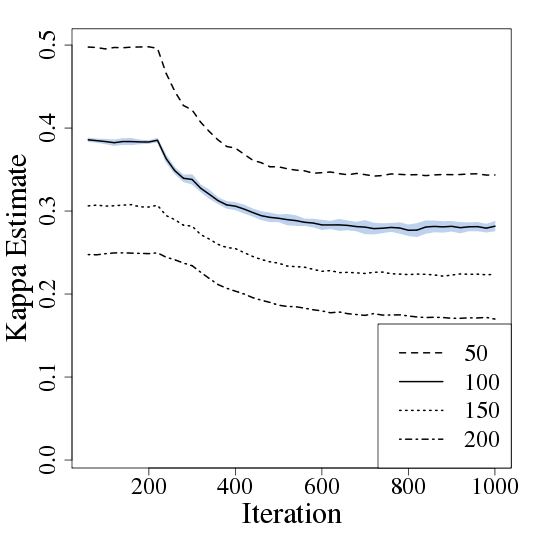
\includegraphics[width=0.45\textwidth]{graphs/ch6/vietnamese-kappa-iters.png}
}
\hfill
\subfloat[Turkish\label{subfig6:kTurkish}]{%
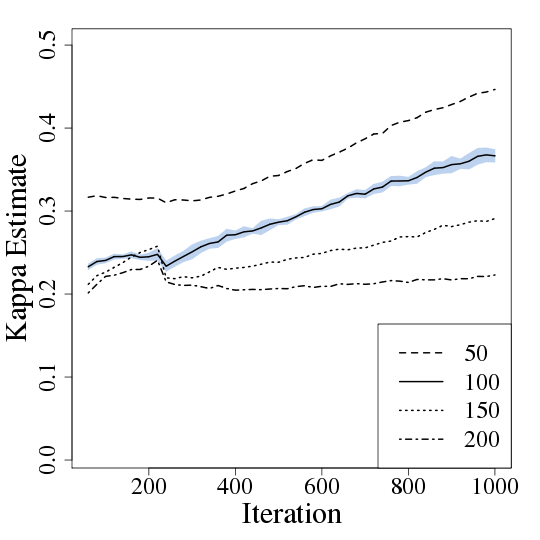
\includegraphics[width=0.45\textwidth]{graphs/ch6/turkish-kappa-iters.png}
}
\end{center}                    
\caption[Convergence and stability of corpus $\kappa$]{Convergence and stability in $\kappa$LDA sampling process for corpus $\kappa$. \label{fig6:kldaKappaIt}}
\end{figure}

We highlight Turkish and Vietnamese as two languages whose repetition behavior we would expect to be most distinct.  Morphologically the two languages are quite different.  Turkish is an agglutanitive language and also exhibits vowel harmony between roots and affixes.  The result of multiple affixes, plus their harmonized forms, applied to a root word results in a large number of distinct word types as compared to other corpora (see \cite{mengusoglu2001} for a discussion of the implications of these properties for speech recognition and language modeling). From our perspective, the addition of affixes may have the effect of turning a word token which could have been a repetition of a previous token into a new word type, lowering the likelihood of repetition.

Vietnamese, by contrast is transcribed at the syllable level and for speech recognition, N-gram language models are also applied at the syllable level, so for purposes of comparison the only available word unit is the syllable.  Although it is sometimes described as `devoid of morphology' \cite{noyer1998vietnamese} many of its units have what Noyer describes as a `reduplicative counterpart' in which the syllable is repeated, perhaps with a change in tone to serve different syntactic or semantic roles.  This, in addition to the combinatorics of a fixed alphabet and small word length limits the number of possible word types and thus increased the likelihood that any particular word type will be repeated in a particular document.

\begin{table}
\begin{center}
   \begin{tabular}{lcccc}
   \textbf{Language}  & $\mathbf{\mathcal{T}=50}$ & \textbf{100} & \textbf{150} & \textbf{200} \\ \midrule
     Tagalog &  0.41 & 0.29 & 0.22 & 0.16 \\
     \rowcolor{blue!5}  Turkish &  0.31 & 0.19 & 0.13 & 0.09 \\
     \rowcolor{blue!5}  Vietnamese & 0.51 & 0.39 & 0.29 & 0.22 \\
     Zulu & 0.33 & 0.26 & 0.21 & 0.16 \\
     Tamil &  0.36 & 0.27 & 0.18 & 0.14 \\ \bottomrule
        \end{tabular}
\caption[Corpus $\kappa$ inferred from development data]{Corpus $\kappa$ inferred from 10 hour development data, by number of latent topics\label{kappas}}
\end{center}
\end{table} 

Table~\ref{kappas} lists the corpus $\kappa$ values for the Babel development corpora, with Turkish and Vietnamese figures called out. Figure~\ref{fig6:devKappa} shows the same estimates, and include error bars representing 1 sample standard deviation across 5 independent trials.  As we would have expected, for a particular number of latent topics $\mathcal{T}$, the highest $\kappa$ value is inferred from the Vietnamese corpus, and the lowest, indicating least token repetition, is inferred from the Turkish Corpus.  

We compare our $\kappa$ estimates to a simple measure of repetition in each corpus, the percentage of tokens in each document that are repeated (i.e. non-singletons).  
\begin{equation}
Document\,Repetition=\frac{1}{|D|}\sum_{d\in D} \left[ 1-\frac{\text{\# types in }d}{\text{\# tokens in }d}\right]
\end{equation}This better quantifies our intuition about the repetition within the Babel languages, as Zulu, Tamil, and Turkish have both low within-document token repetition and low corpus $\kappa$, while Vietnamese has both high $\kappa$ and a high percentage of token repetition (cf. Figure~\ref{fig6:docRep}).
\begin{figure}
\begin{center}
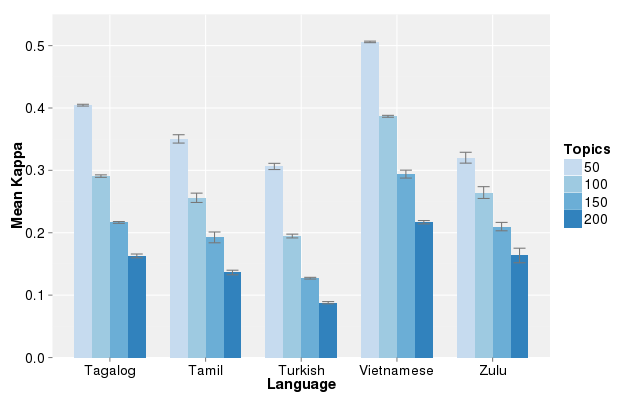
\includegraphics[width=0.7\textwidth]{graphs/ch6/kappas-dev.png}
\end{center}
\caption[Corpus $\kappa$ inferred from development corpora]{Corpus $\kappa$ inferred from development corpora, averaged over 5 sampling runs.\label{fig6:devKappa}}
\end{figure}
\begin{figure}
\begin{center}
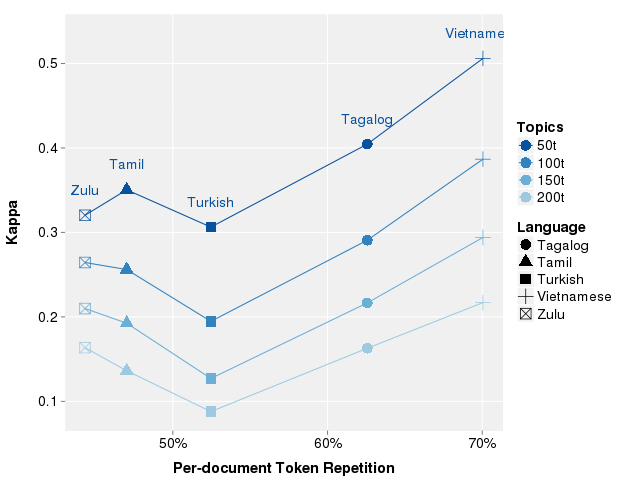
\includegraphics[width=0.7\textwidth]{graphs/ch6/docRep.png}
\end{center}
\caption[Corpus $\kappa$ and per-document token repetition]{Corpus $\kappa$ of development corpora, compared against the percentage of repeated tokens within each document. \label{fig6:docRep}}
\end{figure}

% 
% cd graphs/ch6
% source('corpusRep.R')

\subsection{Document-Level Repetition}

Independent of language, a second property of the model that emerges is the overall decrease in cache usage, as captured by estimated $\kappa$ as the number of latent topics increase.  This is evident in Table~\ref{kappas} and Figures~\ref{fig6:devKappa} and \ref{fig6:docRep}.  We will consider within the context of retrieval in the next chapter to what extent a larger number of topics leads perhaps to overfitting and reducing the need to rely on the cache.  

% cd graphs/ch6
% source('kvar.R')

\begin{figure}
\begin{center}
\subfloat[Zulu\label{subfig6:khistZ}]{%
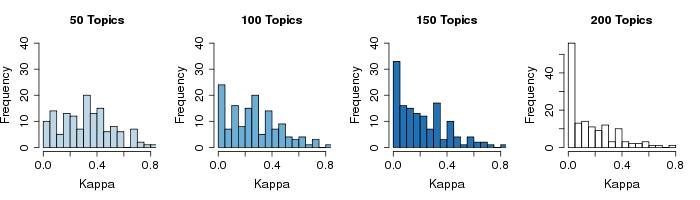
\includegraphics[width=0.7\textwidth]{graphs/ch6/zulu-hist2.png}
}
\\[2ex]
\subfloat[Tamil\label{subfig6:khistTam}]{
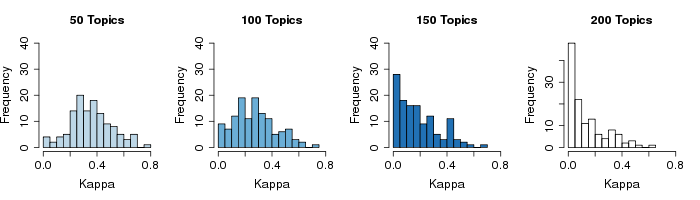
\includegraphics[width=0.7\textwidth]{graphs/ch6/tamil-hist2.png}
}
\\[2ex]
\subfloat[Turkish\label{subfig6:khistTur}]{
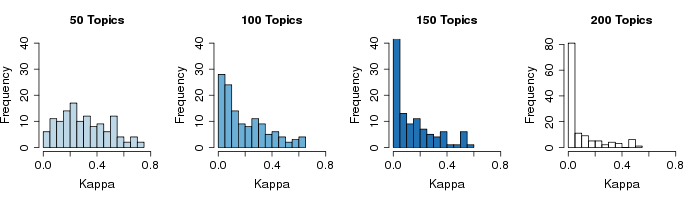
\includegraphics[width=0.7\textwidth]{graphs/ch6/turkish-hist2.png}
}\\[2ex]
\subfloat[Tagalog\label{subfig6:khistTag}]{%
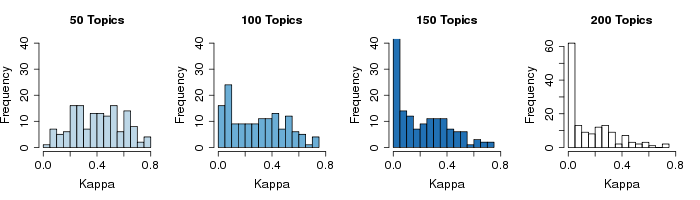
\includegraphics[width=0.7\textwidth]{graphs/ch6/tagalog-hist2.png}
}\\[2ex]
\subfloat[Vietnamese\label{subfig6:khistV}]{
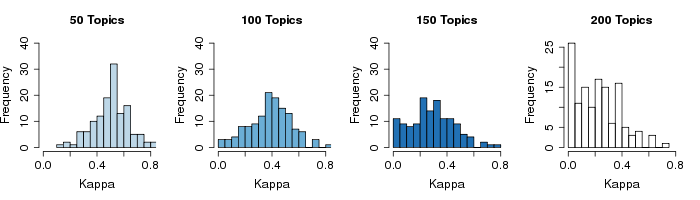
\includegraphics[width=0.7\textwidth]{graphs/ch6/vietnamese-hist2.png}
}
\end{center}
\caption[Histograms of $\kappa^{(d)}$ values]{Histograms of per-document $\kappa^{(d)}$ by language and number of topics $\mathcal{T}$. \label{fig6:khist}}
\end{figure}

We can see the variation by number of latent topics in more detail by shifting our focus from the corpus level $\kappa$ to the per-document estimates of $\kappa^{(d)}$.   If we consider the histograms of the $\kappa^{(d)}$ estimates (cf. Figure~\ref{fig6:khist}) we can see that the variance across individual documents is not insignificant.  Sample standard deviations for the data in Figure~\ref{fig6:khist} is provided in Table~\ref{kappasStdDev}.

\begin{table}[t]
\begin{center}
   \begin{tabular}{lcccc}
   \textbf{Language}  & $\mathbf{\mathcal{T}}$\textbf{=50} & \textbf{100} & \textbf{150} & \textbf{200} \\ \midrule
     Tagalog &  0.18 & 0.20 & 0.19 & 0.18 \\
     Turkish &  0.18 & 0.17 & 0.15 & 0.13 \\
     Vietnamese & 0.13 & 0.16 & 0.16 & 0.16 \\
     Zulu & 0.20 & 0.19 & 0.18 & 0.17 \\
     Tamil &  0.15 & 0.16 & 0.15 & 0.14 \\ \bottomrule
        \end{tabular}
\caption[Sample std. dev. of $\kappa^{(d)}$ estimates across documents ]{Sample standard deviation of $\kappa^{(d)}$ estimates across documents from 10 hour development data by number of topics $\mathcal{T}$\label{kappasStdDev}}
\end{center}
\end{table}   


\subsection{Cached Word Types}
To finish our analysis of the repetition patterns that are learned by our proposed model we look at the individual cache state assignments.  Recall that during the generative process, each word in the corpus is assigned a latent state variable, $k_{d,i}$, indicating whether the word $w_{d,i}$ is to be sampled from the a latent topic or from the current document's cache.  We consider models trained on the Fisher Spanish and English corpora in order to examine which word types are most frequently inferred as having been drawn from the cache ($k_{d,i}=1$).

We focus on the sampler state after 1000 iterations.  Each token in the training corpus is associated with a state value of $k_{d,i}=0$ or $k_{d,i}=1$.  For each word $v$ in the corpus vocabulary we count the number of tokens of that word type assigned a value of 1.  We can define the \textit{cache token count} (CC) over the corpus as sampling state precisely as:
\begin{equation}
CC(v) = \sum_{d\in D}\sum_{i=1}^{|d|} I(w_{d,i}=v \land k_{d,i}=1)
\end{equation}
\noindent where $I(\cdot)$ is an indicator function taking a value of 1 when its expression is true and 0 otherwise.  

We can compare this quantity with other frequency measures that we considered in section~\ref{sec:repetitionMeasure}, in particular, corpus frequency ($f_w$ or CF), document frequency (DF), and \textit{burstiness}, which we previously defined as $f_w/DF_w$.  Plotting the cache token count from the final sampling state against the raw corpus frequency for each vocabulary word, we see a strong correlation, but a number of low frequency words have relatively high cache counts (cf. Figure~\ref{subfig6:cacheStates}).  This pattern also emerged when looking at word burstiness (cf. Figure~\ref{subfig6:burstiness}).    

\begin{figure}
\begin{center}
\subfloat[Cache counts\label{subfig6:cacheStates}]{%
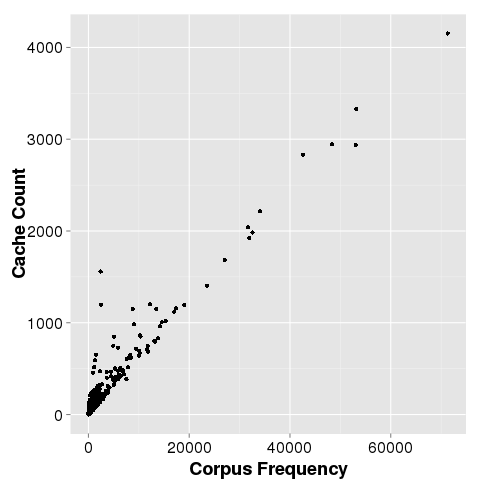
\includegraphics[width=0.4\textwidth]{graphs/ch6/fsp-clda100-1.png}
}
\hfill
\subfloat[Burstiness\label{subfig6:burstiness}]{
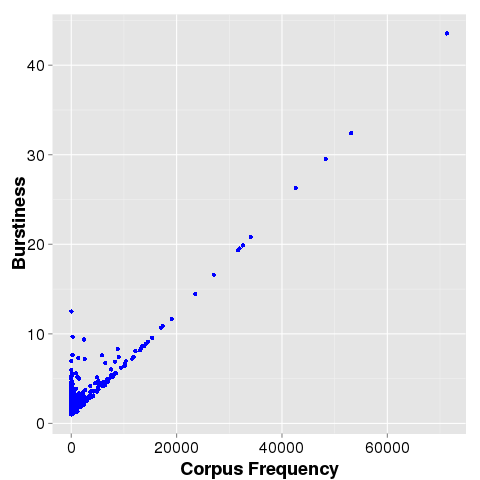
\includegraphics[width=0.4\textwidth]{graphs/ch6/fsp-clda100-2.png}
}
\end{center}
\caption[Measures of repetition for Spanish Words]{Measures of repetition for the Fisher Spanish vocabulary. Each point in the graph represents a word in the training vocabulary. \label{fig6:repSpanish}}
\end{figure}

Again, this phenomenon appears to indicate that we are not just modeling overall frequent words with the cache states.  If we take the words most frequently assigned a cache state (CC Rank) and look at how they are ranked by corpus frequency (CF Rank) and document frequency (DF Rank), irrespective of raw counts, we see that many topic words occur more frequently as cached tokens (cf. Table~\ref{fig6:fspWords}).  The highlighted topic words (chosen from the top 200 cached tokens) are clearly related to various labeled topics within the Fisher collection and occur more frequently by rank in the cache than overall in the corpus by raw or document frequency.
% explains the TF part of IDF

\begin{table}
\begin{center}
\small
\begin{tabular}{l|lccc}
CC Rank & Word & CF Rank & DF Rank & $\chi^2$ Rank\\ \midrule
1 & que & 1 & 6 & 1574 \\
2 & no & 2 & 2 & 1821 \\
3 & de & 4 & 7 & 6241 \\
4 & y & 3 & 1 & 6223 \\
5 & sí & 5 & 12 & 927 \\
6 & la & 6 & 5 & 794 \\
7 & en & 9 & 4 & 1863 \\
8 & es & 7 & 3 & 8112 \\
9 & a & 8 & 8 & 984 \\
10 & yo & 10 & 10 & 3065\\
11 & \textbf{música} & 90 & 368 & 1 \\
\multicolumn{4}{c}{...} \\
46 & \textbf{religión} & 177 & 425 & 2 \\
90 & \textbf{iglesia} & 304 & 566 & 9 \\
98 & \textbf{teléfono} & 176 & 277 & 11991 \\
13 & \textbf{york} & 160 & 190 & 4493 \\
114 & \textbf{nueva} & 154 & 174 & 3147 \\
117 & \textbf{dinero} & 169 & 201 & 860 \\
\multicolumn{4}{c}{ ...} \\
\end{tabular}
\end{center}
\caption[Fisher Spanish words most frequently generated from cache]{Words in Fisher Spanish most frequently assigned a cache state of $k_{d,i}=1$. \label{fig6:fspWords}}
\end{table}


% repeat for english.... 
Although the highlighted frequently cached words are related to the labeled topics, if we compare the CC rank to the $\chi^2$ feature selection metric (cf. \cite{yang1997}) only a few score highly in terms of $\chi^2$ rank.  Indeed if we look across the vocabulary (cf. Figure~\ref{fig6:repSpanish2}), we can see that $\chi^2$ is much more strongly associated with infrequent words, both in terms of DF (Figure~\ref{subfig6:topicCache}) or cache sample frequency (Figure~\ref{subfig6:topicCache}).  

\begin{figure}
\begin{center}
\subfloat[Cache counts\label{subfig6:topicContent}]{%
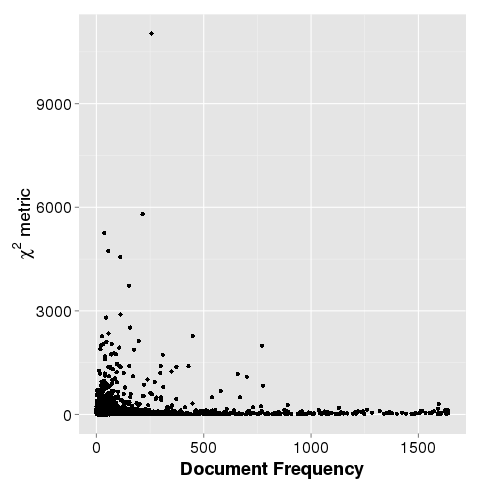
\includegraphics[width=0.45\textwidth]{graphs/ch6/fsp-topic-content.png}
}
\hfill
\subfloat[Burstiness\label{subfig6:topicCache}]{
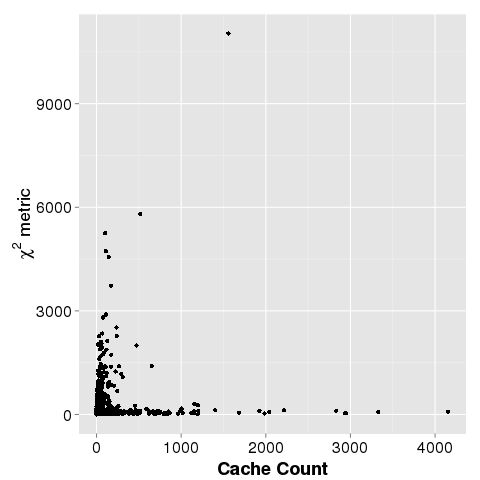
\includegraphics[width=0.45\textwidth]{graphs/ch6/fsp-topic-cache.png}
}
\end{center}
\caption[Topic relevance and repetition of Spanish Words]{Measures of topic relevance and repetition for the Fisher Spanish vocabulary.  Each point in the graph represents a word in the training vocabulary.\label{fig6:repSpanish2}}
\end{figure}

\begin{table}
\begin{center}
\small
\begin{tabular}{l|lccc}
CC Rank & Word & CF Rank & DF Rank & $\chi^2$ Rank\\ \midrule
1 & i & 11 & 1 & 1114 \\
2 & you & 5 & 2 & 913 \\
3 & and & 4 & 3 & 3836 \\
4 & the & 3 & 4 & 1797 \\
5 & yeah & 29 & 8 & 1519 \\
6 & know & 19 & 7 & 750 \\
7 & to & 10 & 5 & 4512 \\
8 & a & 2 & 6 & 1192 \\
9 & that & 9 & 9 & 780 \\
10 & like & 13 & 12 & 1696 \\
\multicolumn{4}{c}{...} \\
73 & \textbf{school} & 213 & 123 & 59 \\
77 & \textbf{watch} & 317 & 160 & 24 \\
84 & \textbf{family} & 269 & 168 & 9 \\
88 & \textbf{minimum} & 1018 & 278 & 2 \\
91 & \textbf{wage} & 1093 & 292 & 1 \\
93 & \textbf{money} & 209 & 129 & 142 \\
95 & \textbf{dog} & 879 & 282 & 4 \\
103 & \textbf{computer} & 506 & 270 & 21 \\
\multicolumn{4}{c}{ ...} \\
\end{tabular}
\end{center}
\caption[Fisher English words most frequently generated from cache]{Words in Fisher English most frequently assigned a cache state of $k_{d,i}=1$. \label{fig6:fshWords}}
\end{table}


If we follow the same analysis for the Fisher English corpus we can observe the same phenomena.  Our proposed cache model captures more than simply frequent words (in terms of corpus or document frequency).  In Table~\ref{fig6:fshWords} we again highlight the content words (indicative of the reference human topic labels) that occur within roughly the top 100 cached words.   Figure~\ref{fig6:repEnglish} contrasts the cached state frequencies to the burstiness measure, showing trends similar to the Spanish corpus.  Likewise, Figure~\ref{fig6:repEnglish2} also shows how words that obtain a high $\chi^2$ score relative to the reference topic labels tend to occur with low document frequency and cache usage.  


\begin{figure}
\begin{center}
\subfloat[Cache counts\label{subfig6:cacheStatesEng}]{%
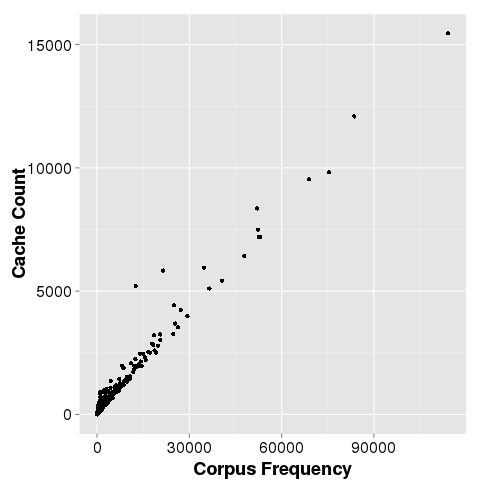
\includegraphics[width=0.4\textwidth]{graphs/ch6/fsh-clda-100-1.png}
}
\hfill
\subfloat[Burstiness\label{subfig6:burstinessEng}]{
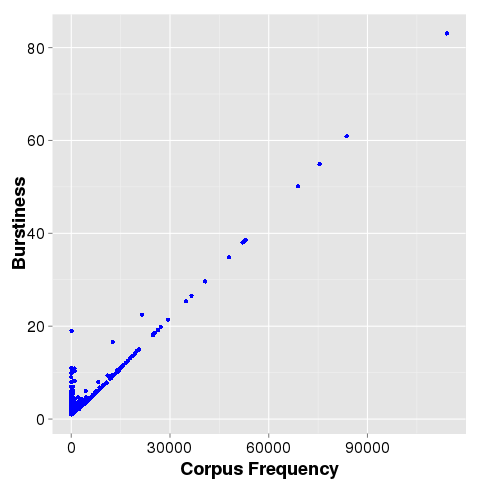
\includegraphics[width=0.4\textwidth]{graphs/ch6/fsh-clda-100-2.png}
}
\end{center}
\caption[Measures of repetition for English Words]{Measures of repetition for the Fisher English vocabulary. Each point in the graph represents a word in the training vocabulary. \label{fig6:repEnglish}}
\end{figure}

\begin{figure}
\begin{center}
\subfloat[Cache counts\label{subfig6:topicContentEng}]{%
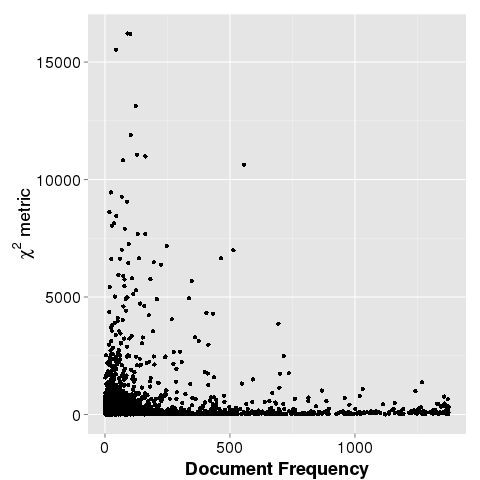
\includegraphics[width=0.45\textwidth]{graphs/ch6/fsh-topic-content.png}
}
\hfill
\subfloat[Burstiness\label{subfig6:topicCacheEng}]{
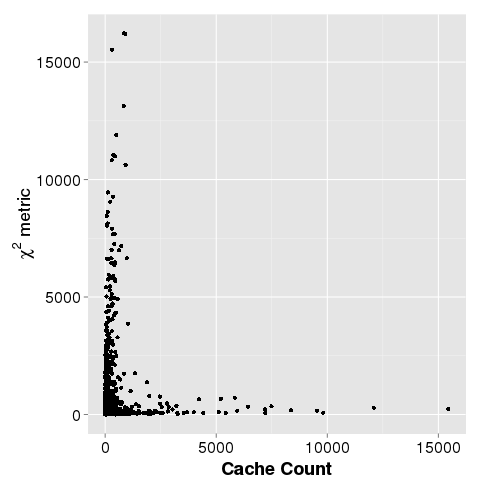
\includegraphics[width=0.45\textwidth]{graphs/ch6/fsh-topic-cache.png}
}
\end{center}
\caption[Topic relevance and repetition of English Words]{Measures of topic relevance and repetition for the Fisher English vocabulary. Each point in the graph represents a word in the training vocabulary. \label{fig6:repEnglish2}}
\end{figure}

Given the examples from the English and Spanish corpora, we can see that the cache state in our model captures unique properties of the given languages:  not simply frequency, not capturing just an additional latent topic.  In the following section we will look at our proposed model as a unigram language model and consider to what effect our modeling of repetition contributes to that task.

\section{Language Models}
Up to this point we have looked primarily at \textit{intrinsic} properties of the model, directly observable or measured from the estimated parameters on our various corpora.  Beginning in this section we begin to shift our focus to external tasks, starting with language modeling.  As we described in the previous chapter, once we have obtained the topic proportions for a document (denoted as $\theta^{(d)}$), it is straightforward to obtain a document-specific unigram language model as a mixture of the topic distributions $\phi^{(t)}$ (cf. Eqn.~\ref{eqn6:unigram}).  

Given the topic distributions and topic proportions we can generate these document-specific unigram LM's either from standard LDA topic models or from our proposed model.  Under our model we can also incorporate the probabilities from the cache frequencies essentially on a word by word basis (cf. Eqns.~\ref{eqn6:cprob},\ref{eqn6:clda}).
\begin{align}
P_d(w_i) =& \sum_{t=1}^T \theta^{(d)}_t \cdot \phi^{(t)}_i \label{eqn6:unigram} \\
P_{cache}{w_i} &= \frac{f_{cache}(w_i)}{\sum_{j=1}^{|V|}f_{cache}(w_j)} \label{eqn6:cprob} \\
P_{d+cache}(w_i) =& \,\kappa^{(d)} P_{cache}(w_i) + (1-\kappa^{(d)}) \cdot  P_{d}(w_i) \label{eqn6:clda}
\end{align}

Given these unigram language models we can look at the performance of LDA and our proposed model in terms of perplexity on the held-out data sets.  Here we take the document-level cache prior $\kappa^{(d)}$ as a natural interpolation weight (Eqn.~\ref{eqn6:clda}).  We contrast the perplexity under three conditions on the 10 hour Babel development corpora.  First, taking the $\theta^{(d)}$ and $\phi^{(t)}$ from standard LDA models, second using only the topic mixtures for our proposed model (denoted $\kappa$LDA$^\prime$), and third, our full proposed unigram model of topic mixtures interpolated with cache probabilities (denoted $\kappa$LDA).

% Do I need to explain perplexity here??

\begin{table}[t]
\centering
   \begin{tabular}{lrrrr}
Language & $\mathcal{T}$ & \textbf{LDA} & \textbf{$\kappa$LDA$^\prime$} & \textbf{$\kappa$LDA} \\ \midrule
 \rowcolor{blue!6} Tagalog & 50   &  142.90  & 163.30 & \textbf{134.43} \\
 \rowcolor{blue!6}& 100  & 136.63 & 153.99 & \textbf{132.35} \\
\rowcolor{blue!6} & 150  & 139.76 & 146.08 & \textbf{130.47} \\
 \rowcolor{blue!6} & 200 & 128.05 & 141.12 & \textbf{129.94} \\[1ex]
 \rowcolor{blue!6} Vietnamese & 50 & 257.94 & 283.52 &  \textbf{217.30} \\
 \rowcolor{blue!6} & 100  & 243.51  & 263.03 & \textbf{210.05} \\
 \rowcolor{blue!6} & 150  & 232.60  & 245.75 & \textbf{205.59} \\
 \rowcolor{blue!6} & 200  & 223.82  & 234.44 &\textbf{204.25} \\[1ex]
Zulu & 50 & \textbf{183.53} & 251.52 & 203.56 \\
& 100  & \textbf{179.44} & 267.42 & 217.11 \\
& 150 & \textbf{174.79} & 269.01 & 223.90 \\
& 200  & \textbf{175.65} & 252.03 & 217.89 \\[1ex] 
Tamil & 50 &\textbf{273.08} & 356.40 & 283.82 \\ 
& 100 & \textbf{265.02} & 369.18 & 297.68 \\ 
& 150 & \textbf{259.42} & 361.79 & 301.92 \\ 
& 200 &\textbf{236.30} & 341.32 &  298.26  \\
Turkish & 50 &\textbf{273.08} & 356.40 & 283.82  \\ 
& 100 & \textbf{265.02} & 369.18 & 297.68 \\ 
& 150 & \textbf{259.42} & 361.79 & 301.92 \\ 
& 200 &\textbf{236.30} & 341.32 &  298.26 \\
\end{tabular}
\caption[Perplexity of topic-mixture unigram LMs]{ Perplexity of topic-mixture unigram language models with and without unigram cache \label{tab6:devppl} }
\end{table}

We can see from Table~\ref{tab6:devppl} that perplexity in general decreases as the number of latent topics $\mathcal{T}$ increases.  However, as we will see in Chapter 7, this is not necessarily predictive of the best retrieval performance.  By themselves, the topic mixtures from our proposed model underperform LDA in terms of perplexity.  However, when the cache probabilities are mixed in, for Tagalog and Vietnamese the perplexity under our proposed model is relatively 3 to 15\% lower than the perplexity under LDA.

\section{Topic Discovery}

While perplexity measures give us a notion of how well our proposed model explains the development data in a general sense, we would like to have some measure of how well our proposed cache-augmented model is able to extract the `subject matter' of the various corpora.  We wish to avoid presenting list of most frequent words in the learned topic distributions, which, though a compelling demonstration of the learning capability of topic models for English, is nonetheless still subjective in nature.  

We will instead extend the analysis followed by May et al (cf. \cite{may2015}) which looks at both the extrinsic performance of topic models as low-dimensional feature representations for classification, but also at the \textit{topic discovery} task, where topic distributions are evaluated as clusterings of the data against a gold standard.  What we find is that in terms of classification performance, our proposed model performs slightly worse than a typical LDA model %HERE 

In order to compare against a gold standard set of topic labels, we restrict the analysis to the labeled LDC Fisher English and Spanish transcripts, with training and testings splits consistent with our previous published work (cf. \cite{wintrode2009,wintrode2013}).   Classification based measures of latent topic models indirectly evaluate the learned topic distributions by posing the question, are the latent topics assigned to each document predictive of the labeled topic in terms of \textit{effective features for classification}?  Cluster-based measures ask the question, are the documents generated from the same latent topics also \textit{assigned the same topic label} by a human annotator?

\subsection{Classification}
% NOTE clean up writing structure, transitions,etc 
In terms of the first question, we use the topic proportions $\theta^{(d)}$ for each document as a $\mathcal{T}$-dimensional feature vector where $\mathcal{T}$ is the number of latent topics.  We extract $\theta^{(d)}$ for our cache-augmented model (denoted $\kappa$LDA) using the Gibbs sampling formulation detailed in Chapter 5.  We also extract $\theta^{(d)}$ using the Mallet implementation of LDA.  Comparison of these two models gives us an indication of what if any ability to capture the subject matter is lost when words are modeled as generated from the cache in our model.   

We train topic models with $\mathcal{T}=\{50,100,200,300,600\}$ under our model and LDA, inferring  $\theta^{(d)}$ for both train and test partitions of the Fisher English and Spanish transcripts.  We train $N$ 1-vs-all binary classifiers, where $N=40$ for Fisher English, and $N=25$ for Fisher Spanish.  All results reported are averaged over all $N$ classifiers.  For a state-of-the art baseline we use TF-IDF weighted bags-of-words features using the full training partition vocabulary in each corpus (26606 and 30170 respectively).  As with previous experiments, we report detection Equal Error Rate (EER), Identification Error Rate (ID Error) and Area Under the recall-precision Curve (AUC) for each system.  General trends are consistent across these metrics, but reflect different application scenarios.


\begin{figure}
\begin{center}
\subfloat[EER\label{subfig6:topicFeatsEER}]{%
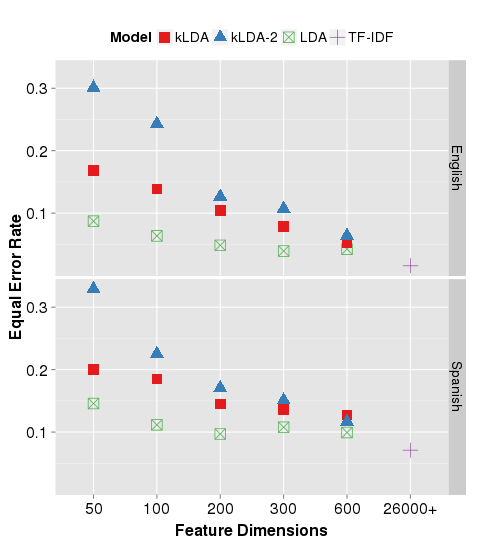
\includegraphics[width=0.45\textwidth]{graphs/ch6/topic-feats.png}
}
\hfill
\subfloat[ID Error\label{subfig6:topicFeatsError}]{%
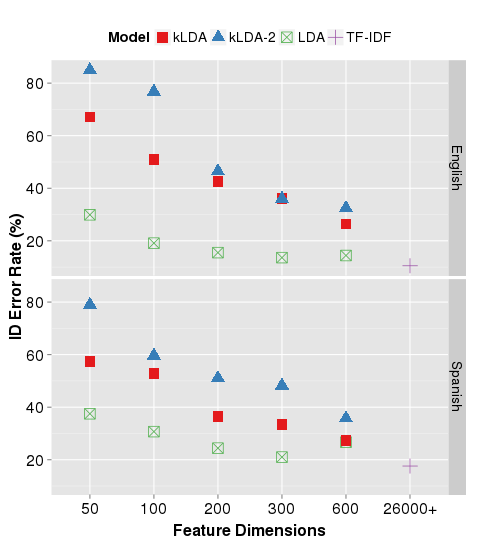
\includegraphics[width=0.45\textwidth]{graphs/ch6/topic-feats-err.png}
} \\
\subfloat[AUC\label{subfig6:topicFeatsAUC}]{%
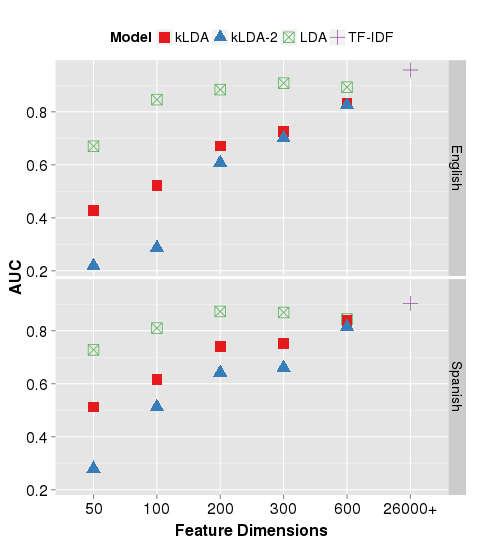
\includegraphics[width=0.45\textwidth]{graphs/ch6/topic-feats-auc.png}
}
\end{center}
\caption[Classification performance using latent topic features]{Classification performance using latent topic features. \label{fig6:topicFeats}}

\end{figure}

We capture the results of both English and Spanish classification tasks in Figure~\ref{fig6:topicFeats}.  From the perspective of classification we can conclude that our cache-augmented model, for all but the largest number of latent topics, lose some ability to capture the labeled topic signal in order to model repetition, vis-à-vis the LDA topic-only model.  This is best visualized as the gap between the performance of the feature vectors $\theta^{(d)}$ inferred from LDA versus $\kappa$LDA and $\kappa$LDA-2 (bigram cache model).

In hindsight the results in Figure~\ref{fig6:topicFeats} follow naturally from the analysis of $\kappa$ estimates in Section~\ref{sec:kldaRepetition}.  As the number of latent topics increase the cache usage decreases, as measured by $\kappa^{(d)}$ for each document (cf. Figure~\ref{fig6:devKappa}).  We might expect the topics learned by our cache-augmented model to approach those learned by the original LDA model as the number of latent topics grows, and from the perspective of classification, this is indeed the case.

It is worth noting again that the classification metrics are an indirect measure of how well the aforementioned models capture `subject matter' behavior, viewed through the lense of a single set of human annotations. The results in Figure~\ref{fig6:topicFeats} suggest that for fewer number latent topics, the cache-augmented models differ significantly from LDA in terms of their discovered topics.  However, if we consider a cluster-based evaluation, we may conclude that this difference in models (LDA versus $\kappa$LDA) is in part application-specific.

\subsection{Clustering}

As in May et al.\cite{may2015}, we also evaluate \textit{topic discovery} of the models in terms of \textit{V-measure} \cite{rosenberg2007}.  V-measure is defined as the harmonic mean of two desirable properties \textit{homogeneity} and \textit{completeness}, similar to F-measure, in which degenerate solutions can result in perfect recall or precision, but not both.  Likewise a degenerate clustering can be obtained where all documents are assigned a single cluster ($c=1$), or where each document is given its own cluster or latent topic ($h=1$).

The formal definitions of homogeneity $h$, completeness $c$, and V-measure $V_\beta$ follow.  V-measure can be parameterized by a $\beta$, a specific preference for $h$ versus $c$.  All of our results report $V_1$ where $\beta=1$ and homogeneity and completeness are weighted equally.  The metric depends on the contingency table $A$ whose entries $a_{ck}$ are the number of documents assigned to class (labeled topic) $c$ and cluster $k$.  As in \cite{may2015} we assign cluster membership based on the most likely latent topic for both LDA and $\kappa$LDA. 

\begin{equation}
V_{\beta} = \frac{\beta+1 \cdot h \cdot c}{\beta \cdot h + c)} 
\end{equation}
\begin{align}
h =&  \begin{cases}
      0 &, \text{if}\ H(C)=0 \\
      1 - \frac{H(C|K)}{H(K)} &, \text{else}
    \end{cases}\\
H(C|K) =& -\sum_{k=1}^{|K|}\sum_{c=1}^{|C|}\frac{a_{ck}}{N}\log\frac{a_{ck}}{\sum_{c=1}^{|C|}a_ck} \\
H(C) =& -\sum_{c=1}^{|C|}\frac{\sum_{k=1}^{|K|}a_{ck}}{N}\log\frac{\sum_{k=1}^{|K|}a_{ck}}{N} \\
c =& 1 - \frac{H(K|C)}{H(K)} \\
H(K|C) =& -\sum_{c=1}^{|C|}\sum_{k=1}^{|K|}\frac{a_{ck}}{N}\log\frac{a_{ck}}{\sum_{k=1}^{|K|}a_ck} \\
H(K) =& -\sum_{k=1}^{|K|}\frac{\sum_{c=1}^{|C|}a_{ck}}{N}\log\frac{\sum_{c=1}^{|C|}a_{ck}}{N}
\end{align}

We use the same topic models from the previous section, trained with $\mathcal{T} = \{50,100,200,300,600\}$. Again we obtain the inferred topic proportions $\theta^{(d)}$ for each document $d$ in the training partition.  Taking the most likely topic $t$ ($\argmax_t \theta^{(d)}_t$) as the cluster assignment for $d$, we compute $V_{1}$ for the topic model induced clustering and some set of class labels $C$ over the training documents.

We consider two choices for class labels.  We can use the human topic labels from the Fisher corpora as a `gold standard' set of classes $C$ for both English and Spanish (where $|C|$ is 40 and 25, respectively).  However we can also take an unsupervised clustering of the transcript bags-of-words as an alternate set of classes.  For the latter comparison, we compute clusters on the training data for each corpus of sizes $|C|=\{25,50,100\}$.  The latter approach is a viable measure when we have no ground truth topic labels.  All of the bags-of-words clustering against which we compare were generated from the training transcripts using the CLUTO toolkit's \cite{cluto} \textit{vcluster} tool with default settings.% and we apply it?

The cluster analysis of the LDA and $\kappa$LDA topic distributions gives a different perspective from the classification task to the question, how well do the models capture topic content in the corpora considered?  Whereas in the classification task, there was a consistent gap between LDA and $\kappa$LDA performance the cluster accuracy with respect to the human class labels (cf. Figure~\ref{subfig6:topicClustLabeled}) is affected by the addition of the cache model for some models but not for all.  Indeed for most of the Spanish models, the $V_1$ performance is similar.  In absolute terms, neither topic model induces clusters as accurate in terms of $V_1$ as a bag-of-words clustering (denoted TF-IDF in Figure~\ref{subfig6:topicClustLabeled}).  

In Figure~\ref{subfig6:topicClustTFIDF} we show the $V_1$ computed in comparing the topic clusters to a bags-of-words clustering of 25, 50, or 100 clusters.  We observe a similar patter in terms of the behavior of $V_1$ given the algorithm and number of topics as compared to the human labeled classes, which we should at the least expect for the English corpus, given the high $V_1$ (0.83) for the bags-of-words versus the human labels.  In all cases, as with the classification task, the bigram $\kappa$LDA ($\kappa$LDA-2) is consistently worse.  

\begin{figure}
\begin{center}
\subfloat[Human labeled topic classes. \label{subfig6:topicClustLabeled}]{%
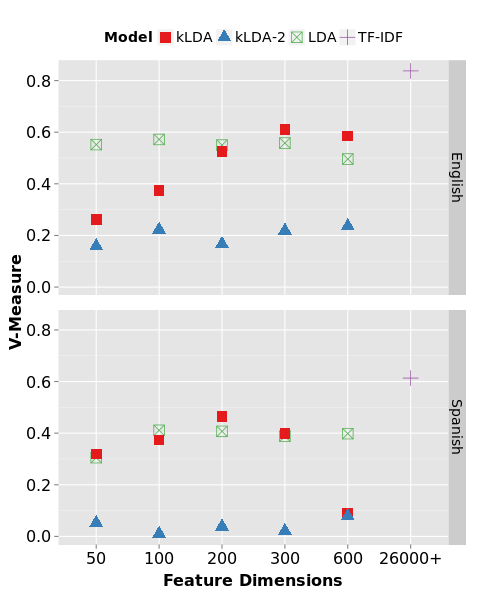
\includegraphics[width=0.4\textwidth]{graphs/ch6/cluster-labeled.png}
}
\hfill
\subfloat[Bag-of-words clustered labels.\label{subfig6:topicClustTFIDF}]{%
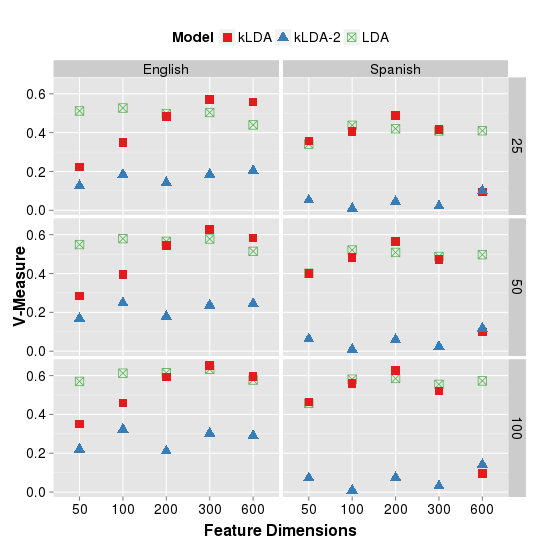
\includegraphics[width=0.5\textwidth]{graphs/ch6/cluster-tfidf.png}
}
\end{center}
\caption[Clustering performance with latent topic features]{Clustering performance with latent topic features. \label{fig6:topicClusts}}

\end{figure}

We can repeat the comparison between the topic-model induced clusters and a bag-of-words clustering on the low-resource IARPA Babel transcripts and observe similar trends as with the larger Fisher corpora.  For the Babel Tagalog, Vietnamese, Zulu, and Tamil training transcripts, we generated reference bag-of-words clusters in the same manner, except for due to the smaller corpus size we looked at cluster sizes of $|C|=\{10,20,30,40\}$.  We used the inferred topics from the models trained using $\mathcal{T}=\{50,100,150,200\}$ latent topics to induce clustering based on the most likely latent topic for each document and computed $V_1$.   The clusering evaluation results for each combination are captured in Figure~\ref{fig6:babelClust}.


\begin{figure}
\centering
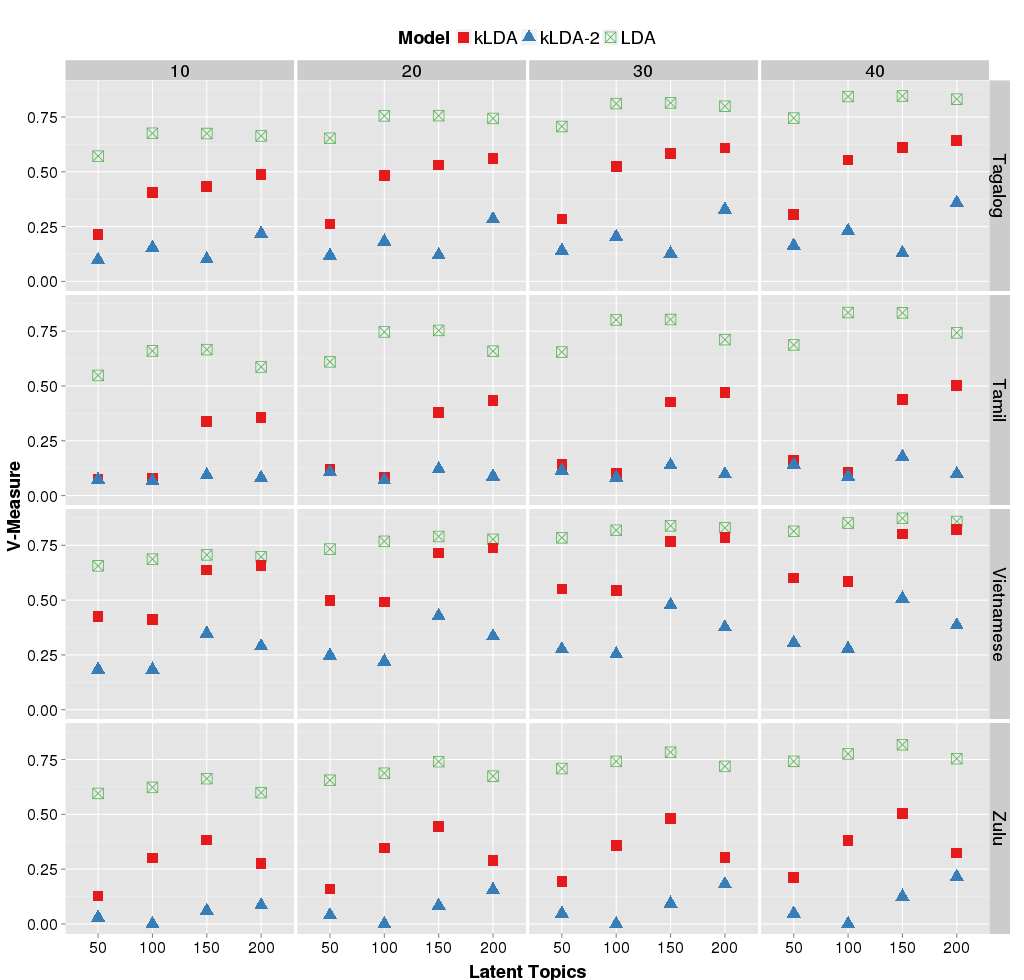
\includegraphics[width=0.9\textwidth]{graphs/ch6/cluster-tfidf-babel.png}
\caption[Clustering evaluation of Babel corpora]{Clustering evaluation of babel corpora \label{fig6:babelClust}}

\end{figure}

In general the bigram $\kappa$LDA models give clusterings that are highly dissimilar to the baseline bag-of-words clusters.  For the unigram cache-augmented model, the similarity with the bag-of-words relative to standard LDA varies by language.  With the exception of Zulu, the clustering performance of the cache-augmented model generally increases with the number of latent topics.  The Vietnamese results stand out particularly, both in terms of the best performing bigram model and in terms of the unigram $\kappa$LDA which at 150 and 200 latent topics, appears to generate topic clusters consistent with standard LDA. 

In conclusion, we can have some confidence that our proposed topic learns similar topic distributions to standard LDA although they do not prove as effective for classification.  The difference in the results between the larger Fisher corpora and the smaller Babel corpora may suggest that the training set size has an effect, but this needs to be separated from language-specific effects.

%we did in fact intend them for the task we consider in the next chapter, which is for language models in speech retrieval.

%finsih decay jobs

\section{Conclusions}

In this chapter we analyzed the behavior of a cache-augmented topic model from a variety of perspectives - model likelihood, cache usage and repetition behavior, perplexity, and topic clustering behavior.   We considered multiple factors which could affect the various metrics, and different facets of our proposed model responded in different degrees to language properties, training size, model parameters such as the number latent topics, and not surprisingly the intended task for each metric.   

In terms of the repetition properties of our proposed models, we observed a number of salient phenomena.  We found that the configured number of latent topics impacted the inferred cache usage (as captured by the $\kappa^{(d)}$ estimate) across all languages.  We also saw that cache usage aligned with what we might expect given intrinsic morphological and other properties of the particular languages.  When we looked at the individual word types that were frequently assigned to the cache state we saw, via English and Spanish examples, that we are not simply replicating word or document frequency properties.

If we focus on the comparison in each case between our proposed model and a standard LDA topic model, we have a mixed set of results in terms of metrics that allow a quantitative comparison such as cluster accuracy, perplexity, or topic classification performance.   Perplexity, for example, is lower under our proposed model in two of the 5 low-resource Babel languages, Tagalog and Vietnamese, which by our metrics, also exhibited the most token repetition.  Similarly, these two languages exhibited the best performance in terms of clustering accuracy (versus standard LDA) when compared with bag-of-word based clusters.

If we consider how much the task affects interpretation of the model performance, for example, when we compare clustering and classification performance, we want to consider carefully each task and topic model combination.  In the next chapter we will do that  by looking specifically at external evaluations of our model in the context of speech recognition and retrieval tasks.  

%3. not as effective for toipc ID as LDA, which in turn does not beat raw bags of words

%4.  but, in some cases discovers similar topics to LDA


